\section{\texorpdfstring{
\includegraphics[width=150pt]{react.png}}{React}}

\begin{frame}

  \frametitle{React}

  JavaScript library for building user interfaces

  React lets you express how your app should look at any given point, and can automatically manage all UI updates when your underlying data changes.

  Is declarative, which means that React conceptually hits the “refresh” button any time data changes, and knows to only update the changed parts

\end{frame}

\begin{frame}[fragile]

  \frametitle{React}

  HTML
  \begin{minted}[fontsize=\tiny]{javascript}
  <body>
    <div id="app"> </div>
    <script src="./bundle.js"></script>
  </body>
  \end{minted}

  index.jsx
  \begin{minted}[fontsize=\tiny]{javascript}
  import './main.css'
  import React from 'react'
  import { render } from 'react-dom'
  import App from './components/App.jsx'

  render(<App name='Social Point' />, document.getElementById('app'))
  \end{minted}

  App.jsx
  \begin{minted}[fontsize=\tiny]{javascript}
  import React from 'react'

  export default class App extends React.Component {
    render () {
      return (
        <div> Hello {this.props.name} </div>
      )
    }
  }
  \end{minted}

\end{frame}

\begin{frame}[fragile]

  \frametitle{Components}
  \mint{javascript}|<App name='Ainara' />|

  es5
  \begin{minted}[fontsize=\tiny]{javascript}
  var App = React.createClass({
    render: function () {
      return <div> Hello {this.props.name} </div>;
    }
  });
  \end{minted}

  es6 class
  \begin{minted}[fontsize=\tiny]{javascript}
  class App extends React.Component {
    render () {
      return (
        <div> Hello {this.props.name} </div>
      )
    }
  }
  \end{minted}

  Stateless
  \begin{minted}[fontsize=\tiny]{javascript}
  const App = props => {
      return <div> Hello {props.name} </div>
  }
  \end{minted}

\end{frame}


\begin{frame}[fragile]

  \frametitle{JSX}

  JSX
  \begin{minted}[fontsize=\tiny]{javascript}
  class App extends React.Component {
    render () {
      return (
        <div> Hello {this.props.name} </div>
      )
    }
  }
  \end{minted}


  Compile js
  \begin{minted}[fontsize=\tiny]{javascript}
  class App extends React.Component {
    render () {
      return React.createElement(
        "div",
        null,
        "Hello ",
        this.props.name
      )
    }
  }
  \end{minted}

\end{frame}

\begin{frame}

  \frametitle{Virtual Dom}

  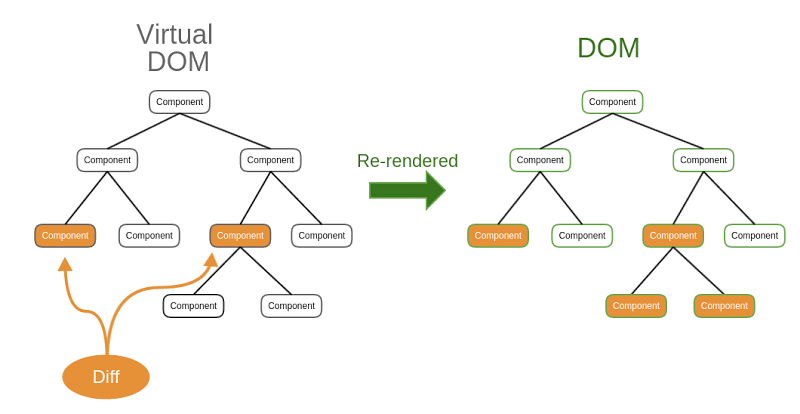
\includegraphics[width=\textwidth]{virtual-dom-update2.png}

\end{frame}

\begin{frame}[fragile]

  \frametitle{Anatomy of components}
  \textbf{render()}

  \small It returns a single child element, either a virtual representation of a native DOM component or another composite component that you've defined yourself. This method is required.

  \textbf{props}
  \begin{minted}[fontsize=\tiny]{javascript}
  class App extends React.Component {
    static propTypes = {
      name: React.PropTypes.string.isRequired
    }

    static defaultProps = {
      name: 'Stranger'
    }

    render () {
      return <div> Hello {this.props.name} </div>
    }
  }

  render(<App name='Alejandro' />, document.getElementById('app'))
  \end{minted}

\end{frame}

\begin{frame}[fragile]

  \frametitle{Anatomy of components}

  \textbf{State}
  \begin{minted}[fontsize=\tiny]{javascript}
  class App extends React.Component {
    constructor (props) {
      super(props)
      // We have to manually bind class methods to maintain the 'this' reference
      this.increaseCounter = this.increaseCounter.bind(this)
      this.state = {
        counter: 0
      }
    }

    increaseCounter (event) {
      this.setState({ counter: this.state.counter++ })  // setState triggers a render()
    }

    render () {
      return (
        <div>
          {this.state.counter}
          <Button onClick={this.increaseCounter}>
            {this.props.name} click here and increase the counter
          </Button>)
        </div>
      )
    }
  }
  \end{minted}

\end{frame}

\begin{frame}[fragile]

  \frametitle{Lifecycle methods}
  \textbf{componentWillMount()}

  \small Invoked before the initial render. Calling \textit{setState} here will not trigger additional renders.

  \textbf{componentDidMount()}

  \small Invoked once after the initial render. Real DOM ref exist in this stage.  Use for integration with other frameworks, timeouts, ajax call, etc.

  \textbf{componentWillReceiveProps(oldProps)}

  \small Invoked when a component is receiving new props. Used to update state on prop changes.
  \begin{minted}[fontsize=\tiny]{javascript}
  componentWillRecieveProps (oldProps) {
    this.setState({  // Does not trigger additional renders
      didIncrease: oldProps.value > this.props.value
    })
  }
  \end{minted}

\end{frame}

\begin{frame}[fragile]

  \frametitle{Lifecycle methods}
  \textbf{shouldComponentUpdate(nextProps, nextState)}

  \small Invoked before rendering before a new state or props changed. If false is returned the component will skip the render method.

  \textbf{componentWillUpdate()}

  \small Invoked immediately before rendering when new props or state are being received. You cannot use \textit{this.setState()}.

  \textbf{componentDidUpdate()}

  \small Invoked immediately after the component's updates are flushed to the DOM.

  \textbf{componentWillUnmount()}

  \small Invoked immediately before a component is unmounted from the DOM. Used for cleanups.

\end{frame}

\begin{frame}[fragile]

  \frametitle{Lifecycle methods}

  \begin{minted}[fontsize=\tiny]{javascript}

  class Timer extends React.Component {
    constructor (props) {
      super(props)
      this.state = { secondsElapsed: 0 }
      // We only have to manually bind the tick method
      // the lifecycle methods are binded automatically by React.
      this.tick = this.tick.bind(this)
    }

    tick () {
      this.setState((prevState) => ({
        secondsElapsed: prevState.secondsElapsed + 1
      }))
    }

    componentDidMount () {
      this.interval = setInterval(() => this.tick(), 1000)
    }

    componentWillUnmount () {
      clearInterval(this.interval)
    }

    render () {
      return <div> Seconds Elapsed: {this.state.secondsElapsed} </div>
    }
  }

  \end{minted}

\end{frame}

\begin{frame}[fragile]

  \frametitle{Events}

  \textbf{SyntheticEvent} is a cross-browser wrapper around the browser's native event. They share the same API, except the wrapper work identically across all browsers.

  \begin{footnotesize}
  \begin{multicols}{5}

    \textbf{Clipboard}

    onCopy

    onCut

    onPaste

    \columnbreak

    \textbf{Keyboard}

    onKeyDown

    onKeyPress

    onKeyUp

    \columnbreak

    \textbf{Focus}

    onFocus

    onBlur

    \columnbreak

    \textbf{Form}

    onChange

    onInput

    onSubmit

    \columnbreak

    \textbf{Mouse}

    onClick

    onContextMenu

    ...

  \end{multicols}
  \end{footnotesize}
  \begin{minted}[fontsize=\tiny]{javascript}
    ...
    increaseCounter (event) {
      this.setState({ counter: this.state.counter++ })
    }
    ...
    render () { return <Button onClick={this.increaseCounter}> Increase </Button> }
    ...
  \end{minted}
\end{frame}

\begin{frame}[fragile]
  \frametitle{Composition}
  \begin{minted}[fontsize=\tiny]{javascript}
  import MyComponent from './MyComponent.jsx'
  ...
    render () {
      const x = 42
      // key is a unique identifier that's required in arrays of components
      const componentsList = [
        <span key='1'> This will render </span>,
        <MyComponent key='2' text='asdf' />
      ]
      return (
        <div>
          <MyComponent prop1={x} {...this.props} />  // Renders MyComponent

          {componentsList}  // Renders all the components in the array

          {null}  // Renders a <noscript> tag
          {false}  // Renders a <noscript> tag
          {this.props.anwser === x && <p> Correct Anwser </p> }

          {[ 'Alejandro', 'Ivan', 'Yisus' ].map(name => {
            if (name === 'Yisus') {
              return null
            }
            let text = `Hello ${name}`
            return <p key=text> {text} </p>
          })}
        </div>
      )
    }
  \end{minted}
\end{frame}

\begin{frame}[fragile]

  \frametitle{Controlled components}

  \begin{minted}[fontsize=\tiny]{javascript}
  class MyForm extends React.Component {
    constructor (props) {
      super(props)
      this.state = { value: 'Hello!' }
      this.handleChange = this.handleChange.bind(this)
    }

    handleChange (event) {
      // Every time the user enters a new character we update the component
      // otherwise he will not see the changes
      this.setState({ value: event.target.value })
    }

    render () {
      return (
        <input
          type="text"
          value={this.state.value}
          onChange={this.handleChange}
        />
      )
    }
  }
  \end{minted}

\end{frame}
